\documentclass[a4paper,10.5pt]{ltjsarticle}
\usepackage{graphicx}
\usepackage{luatexja-fontspec}
\usepackage{caption}
\usepackage{amsmath,amssymb,bm,braket}
\usepackage{gnuplot-lua-tikz}
\usepackage[top=10truemm,bottom=15truemm,left=10truemm,right=10truemm]{geometry}
\usepackage{array}
\usepackage{upgreek}
\usepackage{fancyhdr}
\renewcommand{\refname}{}
\usepackage{listings,jvlisting}
\usepackage{tikz}
\usetikzlibrary{external}
\tikzexternalize
\lstset{
  basicstyle={\ttfamily},
  identifierstyle={\small},
  commentstyle={\smallitshape},
  keywordstyle={\small\bfseries},
  ndkeywordstyle={\small},
  stringstyle={\small\ttfamily},
  frame={tb},
  breaklines=true,
  columns=[l]{fullflexible},
  numbers=left,
  xrightmargin=0pt,
  xleftmargin=3pt,
  numberstyle={\scriptsize},
  stepnumber=1,
  numbersep=1pt,
  lineskip=-0.5ex
}
\captionsetup[figure]{format=plain, labelformat=simple, labelsep=quad,labelfont=bf}
\captionsetup[table]{format=plain, labelformat=simple, labelsep=quad,labelfont=bf}
\parindent = 0pt
\setmainjfont[BoldFont=HiraMinProN-W6]{HiraMinPro-W3}
%[BoldFont=HGSMinchoE]{MSMincho}[BoldFont=HiraMinProN-W6]{HiraMinPro-W3}
\begin{document}
\centerline{\HUGE \bfseries 物理情報工学CD実験 報告書}
\centerline{ }
\rightline{\vspace{-3mm} \Large 2023年度   }
\begin{table}[h]
  \newcolumntype{I}{!{\vrule width 1.5pt}}
  \newcolumntype{i}{!{\vrule width 0.8pt}}
  \arrayrulewidth=0.8pt
  \renewcommand{\arraystretch}{1.5}
  \newcommand{\bhline}[1]{\noalign{\hrule height #1}}
  \huge
  \centering
  \begin{tabular}{Iwc{6cm}Iwc{2cm}iciwc{5cm}I}
    \bhline{1.5pt}
    実験テーマ&\multicolumn{3}{cI}{D4\ AD/DA変換回路}\\
    \hline
    担当教員名&\multicolumn{3}{cI}{増田}\\
    \hline
    実験整理番号&80&実験者氏名&平井 優我\\
    \hline
    共同実験者氏名&\multicolumn{3}{cI}{藤井\ 大樹}\\
    \hline
    曜日組&木&実験日&12月14日\\
    \hline
    実験回&8&報告書提出日&12月20日\\
    \bhline{1.5pt}
  \end{tabular}
\end{table}
\clearpage
%1-2-------------------------------------------------------------------------
\hspace{-2pt}{\Large \bfseries 1.目的}\\
 デジタル信号の特徴を理解すると共に、アナログ信号のデジタル処理に必要なアナログ・デジタル変換の方法と性質を、実験を通じて理解する。\\
\\
\hspace{-2pt}{\Large \bfseries 2.結果と考察}\\
{\large \bfseries 2.1 実験1}\\
 図\ref{A_D}にサンプルホールド波形(緑)、図\ref{D_A}にLPF通過波形(緑)を示す。ただし、黄色の波形は入力正弦波を表す。
\begin{figure}[h]
  \centering
  \begin{minipage}[h]{0.45\linewidth}
    \includegraphics[scale=0.18]{JOUON01.eps}
    \caption*{(a)}
  \end{minipage}
  \begin{minipage}[h]{0.43\linewidth}
    \includegraphics[scale=0.18]{JOUON02.eps}
    \caption*{(b)}
  \end{minipage}
  \begin{minipage}[h]{0.45\linewidth}
    \includegraphics[scale=0.18]{JOUON03.eps}
    \caption*{(c)}
  \end{minipage}
  \begin{minipage}[h]{0.43\linewidth}
    \includegraphics[scale=0.18]{JOUON04.eps}
    \caption*{(d)}
  \end{minipage}
  \caption{アナログ波形をデジタル波形にしたグラフ\ サンプリング周波数(a)$10\ \mathrm{kHz}$\ (b)$5\ \mathrm{kHz}$\ (c)$2\ \mathrm{kHz}$\ (d)$1\ \mathrm{kHz}$}
  \label{A_D}
\end{figure}\\
図\ref{A_D}から、サンプリング周波数を大きくすればするほどサンプルホールド波形は入力正弦波に近い形となった。また、サンプルホールド波形は入力正弦波と位相が一致した。そして、サンプルホールド波形は値が一定となるような部分の数が周波数に比例して変化しているため妥当な形となった。
\clearpage
\begin{figure}[h]
  \centering
  \begin{minipage}[h]{0.45\linewidth}
    \includegraphics[scale=0.18]{JOUON05.eps}
    \caption*{(a)}
  \end{minipage}
  \begin{minipage}[h]{0.43\linewidth}
    \includegraphics[scale=0.18]{JOUON06.eps}
    \caption*{(b)}
  \end{minipage}
  \begin{minipage}[h]{0.45\linewidth}
    \includegraphics[scale=0.18]{JOUON07.eps}
    \caption*{(c)}
  \end{minipage}
  \begin{minipage}[h]{0.43\linewidth}
    \includegraphics[scale=0.18]{JOUON08.eps}
    \caption*{(d)}
  \end{minipage}
  \caption{デジタル波形をアナログ波形にしたグラフ\ サンプリング周波数(a)$10\ \mathrm{kHz}$\ (b)$5\ \mathrm{kHz}$\ (c)$2\ \mathrm{kHz}$\ (d)$1\ \mathrm{kHz}$}
  \label{D_A}
\end{figure}
図\ref{D_A}から、サンプリング周波数が$10,5,2\ \mathrm{kHz}$のとき、LPF通過波形は入力正弦波に近い形となった。これより、アナログ波形の周波数$1\ \mathrm{kHz}$の2倍以上のサンプリング周波数だと、LPF通過波形が入力正弦に近い形となり、サンプリング定理が成り立っている。また、LPF通過波形は入力波形よりも位相が早くなった。そして、LPF通過波形はサンプルホールド波形の急激に値が変化した部分をなめらかにしたような波形となった。\\
 周波数を連続的に変化させたときにサンプルホールド波形とLPF通過波形がどのように変化するかを考える。まず、サンプルホールド波形について、周波数を大きくすると値が一定となる部分が小さくなり入力正弦波に近づいていくと考えられる。逆に周波数を小さくするとき、入力波形をそのままサンプリングする部分とその値をホールドする部分が長くなっていき、元の入力波形と一定値が交互に繰り返されるような波形となる。\\
 図\ref{A_D}について、振幅の減衰と位相差を見積もると表\ref{ADattenuation-delay}となる。
\begin{table}[h]
  \newcolumntype{I}{!{\vrule width 1.5pt}}
  \newcolumntype{i}{!{\vrule width 0.5pt}}
  \arrayrulewidth=0.8pt
  \renewcommand{\arraystretch}{1.5}
  \newcommand{\bhline}[1]{\noalign{\hrule height #1}}
  \centering
  \caption{振れ幅の減衰と位相差}
  \label{ADattenuation-delay}
  \begin{tabular}{IciccI}
    \bhline{1.5pt}
    \begin{tabular}{c}
      サンプリング\\[-10pt]
      周波数\ /\ kHz\\
    \end{tabular}
    &振幅の減衰率&位相差\\
    \hline
    10&0.99&$-0.012$\pi\\
    5&1.0&$-0.011\pi$\\
    2&0.86&$-0.0035\pi$\\
    1&0.88&$0.0\pi$\\
    \bhline{1.5pt}
  \end{tabular}
\end{table}
\clearpage
表\ref{ADattenuation-delay}から、サンプリング周波数が5\ kHzよりも小さくなると振幅が減衰することがわかる。これは入力波形の周波数に対してサンプリング周波数が小さく、入力波形で最大振幅が実現される直前の領域で値がホールドされていることに起因する。ただし、サンプリングする位相をずらすことで振幅の減衰率は1になり得る。\\
 次に、図\ref{D_A}について、振幅の減衰と位相差を見積もると表\ref{DAattenuation-delay}となる。
\begin{table}[h]
  \newcolumntype{I}{!{\vrule width 1.5pt}}
  \newcolumntype{i}{!{\vrule width 0.5pt}}
  \arrayrulewidth=0.8pt
  \renewcommand{\arraystretch}{1.5}
  \newcommand{\bhline}[1]{\noalign{\hrule height #1}}
  \centering
  \caption{振れ幅の減衰と位相差}
  \label{DAattenuation-delay}
  \begin{tabular}{IciccI}
    \bhline{1.5pt}
    \begin{tabular}{c}
      サンプリング\\[-10pt]
      周波数\ /\ kHz\\
    \end{tabular}
    &振幅の減衰率&位相差\\
    \hline
    10&0.49&$-0.54\pi$\\
    5&0.49&$-0.54\pi$\\
    2&0.50&$-0.50\pi$\\
    1&0.47&$-0.64\pi$\\
    \bhline{1.5pt}
  \end{tabular}
\end{table}\\
 表\ref{DAattenuation-delay}から、振幅の減衰率はサンプリング周波数によらず約$-6$\ dBなり、位相差はサンプリング周波数によらず約$\pi/2$となった。これらの結果から位相差も振幅の減衰も理論値とほぼ一致し、表\ref{DAattenuation-delay}の結果は妥当である。\\
 次にFGによって発生される正弦波とパルス波のタイミングのずれについて考える。正弦波とパルス波のタイミングがずれると、サンプルホールドするタイミングがずれることは自明である。これにより、正弦波の山または谷の直前でホールドすればサンプルホールド波形の振幅は小さくなる。逆に、正弦波の山または谷の直後でホールドすればサンプルホールド波形の振幅は入力正弦波に一致する。\\
\\
{\large \bfseries 2.2 実験2}\\
{\large \bfseries 2.2.1\ DA変換}\\
 図\ref{DA}に入力と出力の関係を示す。ただし、点は測定値、黒線は測定点を直線で繋いだ線、赤の破線は原点と$(256,5)$を繋ぐ直線を表す。\\
\begin{figure}[h]
  \centering
  \scalebox{0.45}[0.45]{
\begin{tikzpicture}[gnuplot]
%% generated with GNUPLOT 5.4p10 (Lua 5.4; terminal rev. Jun 2020, script rev. 118)
%% Sun Nov 12 18:33:30 2023
\path (0.000,0.000) rectangle (12.500,8.750);
\gpcolor{color=gp lt color border}
\gpsetlinetype{gp lt border}
\gpsetdashtype{gp dt solid}
\gpsetlinewidth{1.00}
\draw[gp path] (0.018,0.031)--(0.198,0.031);
\draw[gp path] (12.480,0.031)--(12.300,0.031);
\node[gp node right] at (-0.166,0.031) {$15$};
\draw[gp path] (0.018,1.479)--(0.198,1.479);
\draw[gp path] (12.480,1.479)--(12.300,1.479);
\node[gp node right] at (-0.166,1.479) {$20$};
\draw[gp path] (0.018,2.927)--(0.198,2.927);
\draw[gp path] (12.480,2.927)--(12.300,2.927);
\node[gp node right] at (-0.166,2.927) {$25$};
\draw[gp path] (0.018,4.375)--(0.198,4.375);
\draw[gp path] (12.480,4.375)--(12.300,4.375);
\node[gp node right] at (-0.166,4.375) {$30$};
\draw[gp path] (0.018,5.822)--(0.198,5.822);
\draw[gp path] (12.480,5.822)--(12.300,5.822);
\node[gp node right] at (-0.166,5.822) {$35$};
\draw[gp path] (0.018,7.270)--(0.198,7.270);
\draw[gp path] (12.480,7.270)--(12.300,7.270);
\node[gp node right] at (-0.166,7.270) {$40$};
\draw[gp path] (0.018,8.718)--(0.198,8.718);
\draw[gp path] (12.480,8.718)--(12.300,8.718);
\node[gp node right] at (-0.166,8.718) {$45$};
\draw[gp path] (0.018,0.031)--(0.018,0.211);
\draw[gp path] (0.018,8.718)--(0.018,8.538);
\node[gp node center] at (0.018,-0.277) {$0$};
\draw[gp path] (1.935,0.031)--(1.935,0.211);
\draw[gp path] (1.935,8.718)--(1.935,8.538);
\node[gp node center] at (1.935,-0.277) {$0.2$};
\draw[gp path] (3.852,0.031)--(3.852,0.211);
\draw[gp path] (3.852,8.718)--(3.852,8.538);
\node[gp node center] at (3.852,-0.277) {$0.4$};
\draw[gp path] (5.770,0.031)--(5.770,0.211);
\draw[gp path] (5.770,8.718)--(5.770,8.538);
\node[gp node center] at (5.770,-0.277) {$0.6$};
\draw[gp path] (7.687,0.031)--(7.687,0.211);
\draw[gp path] (7.687,8.718)--(7.687,8.538);
\node[gp node center] at (7.687,-0.277) {$0.8$};
\draw[gp path] (9.604,0.031)--(9.604,0.211);
\draw[gp path] (9.604,8.718)--(9.604,8.538);
\node[gp node center] at (9.604,-0.277) {$1$};
\draw[gp path] (11.521,0.031)--(11.521,0.211);
\draw[gp path] (11.521,8.718)--(11.521,8.538);
\node[gp node center] at (11.521,-0.277) {$1.2$};
\draw[gp path] (0.018,8.718)--(0.018,0.031)--(12.480,0.031)--(12.480,8.718)--cycle;
\node[gp node center,rotate=-270] at (-0.826,4.374) {$J$};
\node[gp node center] at (6.249,-0.738) {$F^*$};
\gpcolor{rgb color={0.000,0.000,0.000}}
\gpsetlinewidth{5.00}
\draw[gp path] (0.977,8.142)--(1.935,3.417)--(2.894,1.542)--(3.852,0.700)--(4.811,0.321)%
  --(5.770,0.196)--(5.943,0.194)--(6.728,0.244)--(7.687,0.429)--(8.646,0.742)--(9.604,1.189)%
  --(10.563,1.795)--(11.521,2.601);
\gpsetpointsize{3.20}
\gp3point{gp mark 7}{}{(0.977,8.142)}
\gp3point{gp mark 7}{}{(1.935,3.417)}
\gp3point{gp mark 7}{}{(2.894,1.542)}
\gp3point{gp mark 7}{}{(3.852,0.700)}
\gp3point{gp mark 7}{}{(4.811,0.321)}
\gp3point{gp mark 7}{}{(5.770,0.196)}
\gp3point{gp mark 7}{}{(5.943,0.194)}
\gp3point{gp mark 7}{}{(6.728,0.244)}
\gp3point{gp mark 7}{}{(7.687,0.429)}
\gp3point{gp mark 7}{}{(8.646,0.742)}
\gp3point{gp mark 7}{}{(9.604,1.189)}
\gp3point{gp mark 7}{}{(10.563,1.795)}
\gp3point{gp mark 7}{}{(11.521,2.601)}
\gpcolor{color=gp lt color border}
\gpsetlinewidth{1.00}
\draw[gp path] (0.018,8.718)--(0.018,0.031)--(12.480,0.031)--(12.480,8.718)--cycle;
%% coordinates of the plot area
\gpdefrectangularnode{gp plot 1}{\pgfpoint{0.018cm}{0.031cm}}{\pgfpoint{12.480cm}{8.718cm}}
\end{tikzpicture}
}

  \vspace{-30pt}\caption{入出力の関係}
  \label{DA}
\end{figure}\\
理論値は、
\begin{align}
  V_\mathrm{out}=\Delta\times\sum^{n-1}_{k=0}{d_k\cdot 2^k}\ ,\ \Delta=\frac{E_\mathrm{ref}}{2^n}\ ,\ d_k=0\ \mathrm{or}\ 1
\end{align}
から、赤の破線と一致すると考えられる。また、赤の破線の傾きの値$0.020$はデジタル値が1増加したときのアナログ電圧の増加量を表す。図\ref{DA}から、測定値は全体的に赤の破線よりも値が小さくなり、理論値からの値の減少は入力したデジタル値が大きくなるほど大きくなった。この誤差の原因としては回路内の抵抗が考えられる。
 ここで、上記で示した誤差を小さくする方法を提示する。まず、測定点の回帰直線を求めるとその傾きは0.018である。ただし、回帰直線は原点を通る前提とした。これより、出力されるアナログ電圧の理論値と測定値の比は大まかに$0.02/0.018=1.1$である。よって、巻き数の比が1.1:1の変圧器を用いれば理論値とほぼ一致させることができる。\\
 ビット数を大きくすると用いる回路も大きくなることから回路内の誤差も含めた抵抗値は大きくなると考えられる。そのため、出力されるアナログ電圧の理論値と測定値の比$p$は大きくなっていく。仮に$n$ビットDACを用いる場合、出力されるアナログ電圧の理論値と測定値の比は$p(n)$、理論値の直線の傾きは$5/2^n$だから、回帰直線の傾き$a$は、
\begin{align}
  a=\frac{1}{p(n)}\frac{5}{2^n}
\end{align}
と表せる。\\
\\
{\large \bfseries 2.2.2\ AD変換}\\
 図\ref{AD}に入力と出力の関係を示す。ただし、点は測定値、黒線は測定点を直線で繋いだ線、赤の破線は原点と$(5,256)$を繋ぐ直線を表す。\\
\begin{figure}[h]
  \centering
  \scalebox{0.5}[0.5]{
\begin{tikzpicture}[gnuplot]
%% generated with GNUPLOT 5.4p10 (Lua 5.4; terminal rev. Jun 2020, script rev. 118)
%% Sat Dec  9 17:21:03 2023
\path (0.000,0.000) rectangle (12.500,8.750);
\gpcolor{color=gp lt color border}
\gpsetlinetype{gp lt border}
\gpsetdashtype{gp dt solid}
\gpsetlinewidth{1.00}
\draw[gp path] (0.018,0.031)--(0.198,0.031);
\draw[gp path] (12.480,0.031)--(12.300,0.031);
\node[gp node right] at (-0.166,0.031) {$0$};
\draw[gp path] (0.018,0.900)--(0.198,0.900);
\draw[gp path] (12.480,0.900)--(12.300,0.900);
\node[gp node right] at (-0.166,0.900) {$0.1$};
\draw[gp path] (0.018,1.768)--(0.198,1.768);
\draw[gp path] (12.480,1.768)--(12.300,1.768);
\node[gp node right] at (-0.166,1.768) {$0.2$};
\draw[gp path] (0.018,2.637)--(0.198,2.637);
\draw[gp path] (12.480,2.637)--(12.300,2.637);
\node[gp node right] at (-0.166,2.637) {$0.3$};
\draw[gp path] (0.018,3.506)--(0.198,3.506);
\draw[gp path] (12.480,3.506)--(12.300,3.506);
\node[gp node right] at (-0.166,3.506) {$0.4$};
\draw[gp path] (0.018,4.375)--(0.198,4.375);
\draw[gp path] (12.480,4.375)--(12.300,4.375);
\node[gp node right] at (-0.166,4.375) {$0.5$};
\draw[gp path] (0.018,5.243)--(0.198,5.243);
\draw[gp path] (12.480,5.243)--(12.300,5.243);
\node[gp node right] at (-0.166,5.243) {$0.6$};
\draw[gp path] (0.018,6.112)--(0.198,6.112);
\draw[gp path] (12.480,6.112)--(12.300,6.112);
\node[gp node right] at (-0.166,6.112) {$0.7$};
\draw[gp path] (0.018,6.981)--(0.198,6.981);
\draw[gp path] (12.480,6.981)--(12.300,6.981);
\node[gp node right] at (-0.166,6.981) {$0.8$};
\draw[gp path] (0.018,7.849)--(0.198,7.849);
\draw[gp path] (12.480,7.849)--(12.300,7.849);
\node[gp node right] at (-0.166,7.849) {$0.9$};
\draw[gp path] (0.018,8.718)--(0.198,8.718);
\draw[gp path] (12.480,8.718)--(12.300,8.718);
\node[gp node right] at (-0.166,8.718) {$1$};
\draw[gp path] (0.018,0.031)--(0.018,0.211);
\draw[gp path] (0.018,8.718)--(0.018,8.538);
\node[gp node center] at (0.018,-0.277) {$1200$};
\draw[gp path] (1.576,0.031)--(1.576,0.211);
\draw[gp path] (1.576,8.718)--(1.576,8.538);
\node[gp node center] at (1.576,-0.277) {$1250$};
\draw[gp path] (3.134,0.031)--(3.134,0.211);
\draw[gp path] (3.134,8.718)--(3.134,8.538);
\node[gp node center] at (3.134,-0.277) {$1300$};
\draw[gp path] (4.691,0.031)--(4.691,0.211);
\draw[gp path] (4.691,8.718)--(4.691,8.538);
\node[gp node center] at (4.691,-0.277) {$1350$};
\draw[gp path] (6.249,0.031)--(6.249,0.211);
\draw[gp path] (6.249,8.718)--(6.249,8.538);
\node[gp node center] at (6.249,-0.277) {$1400$};
\draw[gp path] (7.807,0.031)--(7.807,0.211);
\draw[gp path] (7.807,8.718)--(7.807,8.538);
\node[gp node center] at (7.807,-0.277) {$1450$};
\draw[gp path] (9.365,0.031)--(9.365,0.211);
\draw[gp path] (9.365,8.718)--(9.365,8.538);
\node[gp node center] at (9.365,-0.277) {$1500$};
\draw[gp path] (10.922,0.031)--(10.922,0.211);
\draw[gp path] (10.922,8.718)--(10.922,8.538);
\node[gp node center] at (10.922,-0.277) {$1550$};
\draw[gp path] (12.480,0.031)--(12.480,0.211);
\draw[gp path] (12.480,8.718)--(12.480,8.538);
\node[gp node center] at (12.480,-0.277) {$1600$};
\draw[gp path] (0.018,8.718)--(0.018,0.031)--(12.480,0.031)--(12.480,8.718)--cycle;
\node[gp node center,rotate=-270,font={\fontsize{17.0pt}{20.4pt}\selectfont}] at (-1.286,4.374) {光強度比$P(r)/P(0)$};
\node[gp node center,font={\fontsize{17.0pt}{20.4pt}\selectfont}] at (6.249,-1.046) {距離$\ /\ \mathrm{\upmu m}$};
\gpcolor{rgb color={0.000,0.000,0.000}}
\draw[gp path] (0.018,0.207)--(0.064,0.221)--(0.110,0.218)--(0.156,0.205)--(0.202,0.205)%
  --(0.248,0.183)--(0.294,0.196)--(0.340,0.210)--(0.386,0.207)--(0.431,0.176)--(0.477,0.212)%
  --(0.523,0.212)--(0.569,0.198)--(0.615,0.210)--(0.661,0.198)--(0.707,0.207)--(0.753,0.203)%
  --(0.799,0.225)--(0.845,0.198)--(0.891,0.223)--(0.937,0.203)--(0.983,0.218)--(1.029,0.205)%
  --(1.075,0.205)--(1.121,0.216)--(1.167,0.203)--(1.213,0.203)--(1.259,0.196)--(1.305,0.212)%
  --(1.351,0.189)--(1.397,0.205)--(1.443,0.216)--(1.489,0.214)--(1.535,0.205)--(1.581,0.207)%
  --(1.627,0.207)--(1.673,0.201)--(1.719,0.221)--(1.765,0.216)--(1.811,0.207)--(1.857,0.207)%
  --(1.903,0.198)--(1.949,0.205)--(1.995,0.205)--(2.041,0.212)--(2.087,0.221)--(2.133,0.210)%
  --(2.179,0.218)--(2.225,0.218)--(2.271,0.225)--(2.317,0.214)--(2.363,0.212)--(2.409,0.205)%
  --(2.455,0.221)--(2.501,0.223)--(2.547,0.227)--(2.593,0.203)--(2.639,0.194)--(2.685,0.210)%
  --(2.731,0.214)--(2.777,0.205)--(2.823,0.194)--(2.869,0.210)--(2.915,0.194)--(2.961,0.212)%
  --(3.007,0.205)--(3.053,0.225)--(3.099,0.223)--(3.145,0.205)--(3.191,0.221)--(3.237,0.216)%
  --(3.283,0.216)--(3.329,0.214)--(3.375,0.212)--(3.420,0.212)--(3.466,0.212)--(3.512,0.212)%
  --(3.558,0.227)--(3.604,0.203)--(3.650,0.207)--(3.696,0.223)--(3.742,0.194)--(3.788,0.212)%
  --(3.834,0.218)--(3.880,0.225)--(3.926,0.207)--(3.972,0.210)--(4.018,0.185)--(4.064,0.223)%
  --(4.110,0.205)--(4.156,0.207)--(4.202,0.218)--(4.248,0.198)--(4.294,0.225)--(4.340,0.216)%
  --(4.386,0.203)--(4.432,0.192)--(4.478,0.187)--(4.524,0.225)--(4.570,0.189)--(4.616,0.212)%
  --(4.662,0.221)--(4.708,0.221)--(4.754,0.203)--(4.800,0.234)--(4.846,0.214)--(4.892,0.223)%
  --(4.938,0.203)--(4.984,0.232)--(5.030,0.210)--(5.076,0.210)--(5.122,0.216)--(5.168,0.203)%
  --(5.214,0.236)--(5.260,0.223)--(5.306,0.227)--(5.352,0.207)--(5.398,0.243)--(5.444,0.225)%
  --(5.490,0.194)--(5.536,0.218)--(5.582,0.245)--(5.628,0.225)--(5.674,0.225)--(5.720,0.214)%
  --(5.766,0.250)--(5.812,0.223)--(5.858,0.261)--(5.904,0.256)--(5.950,0.256)--(5.996,0.301)%
  --(6.042,0.361)--(6.088,0.426)--(6.134,0.553)--(6.180,0.823)--(6.226,1.173)--(6.272,1.707)%
  --(6.318,2.633)--(6.364,3.720)--(6.410,4.612)--(6.455,5.458)--(6.501,5.969)--(6.547,6.634)%
  --(6.593,7.011)--(6.639,7.578)--(6.685,7.774)--(6.731,8.107)--(6.777,8.205)--(6.823,8.339)%
  --(6.869,8.515)--(6.915,8.497)--(6.961,8.444)--(7.007,8.718)--(7.053,8.696)--(7.099,8.611)%
  --(7.145,8.564)--(7.191,8.535)--(7.237,8.479)--(7.283,8.272)--(7.329,7.850)--(7.375,7.522)%
  --(7.421,6.899)--(7.467,6.092)--(7.513,5.137)--(7.559,4.146)--(7.605,2.970)--(7.651,2.124)%
  --(7.697,1.470)--(7.743,1.115)--(7.789,0.841)--(7.835,0.618)--(7.881,0.500)--(7.927,0.386)%
  --(7.973,0.343)--(8.019,0.294)--(8.065,0.281)--(8.111,0.245)--(8.157,0.241)--(8.203,0.203)%
  --(8.249,0.245)--(8.295,0.256)--(8.341,0.205)--(8.387,0.210)--(8.433,0.221)--(8.479,0.230)%
  --(8.525,0.218)--(8.571,0.201)--(8.617,0.216)--(8.663,0.221)--(8.709,0.183)--(8.755,0.218)%
  --(8.801,0.201)--(8.847,0.218)--(8.893,0.212)--(8.939,0.205)--(8.985,0.201)--(9.031,0.218)%
  --(9.077,0.227)--(9.123,0.223)--(9.169,0.218)--(9.215,0.214)--(9.261,0.223)--(9.307,0.198)%
  --(9.353,0.221)--(9.399,0.201)--(9.445,0.216)--(9.490,0.236)--(9.536,0.216)--(9.582,0.203)%
  --(9.628,0.221)--(9.674,0.196)--(9.720,0.207)--(9.766,0.212)--(9.812,0.207)--(9.858,0.196)%
  --(9.904,0.212)--(9.950,0.218)--(9.996,0.198)--(10.042,0.225)--(10.088,0.205)--(10.134,0.216)%
  --(10.180,0.207)--(10.226,0.225)--(10.272,0.212)--(10.318,0.203)--(10.364,0.201)--(10.410,0.214)%
  --(10.456,0.198)--(10.502,0.214)--(10.548,0.205)--(10.594,0.210)--(10.640,0.192)--(10.686,0.225)%
  --(10.732,0.210)--(10.778,0.216)--(10.824,0.210)--(10.870,0.214)--(10.916,0.201)--(10.962,0.207)%
  --(11.008,0.216)--(11.054,0.205)--(11.100,0.212)--(11.146,0.218)--(11.192,0.218)--(11.238,0.210)%
  --(11.284,0.205)--(11.330,0.212)--(11.376,0.198)--(11.422,0.214)--(11.468,0.189)--(11.514,0.214)%
  --(11.560,0.225)--(11.606,0.210)--(11.652,0.225)--(11.698,0.216)--(11.744,0.214)--(11.790,0.214)%
  --(11.836,0.192)--(11.882,0.230)--(11.928,0.205)--(11.974,0.207)--(12.020,0.214)--(12.066,0.218)%
  --(12.112,0.198)--(12.158,0.221)--(12.204,0.201)--(12.250,0.221)--(12.296,0.214)--(12.342,0.210)%
  --(12.388,0.196)--(12.434,0.205)--(12.480,0.207);
\gpsetpointsize{1.20}
\gp3point{gp mark 7}{}{(0.064,0.221)}
\gp3point{gp mark 7}{}{(0.110,0.218)}
\gp3point{gp mark 7}{}{(0.156,0.205)}
\gp3point{gp mark 7}{}{(0.202,0.205)}
\gp3point{gp mark 7}{}{(0.248,0.183)}
\gp3point{gp mark 7}{}{(0.294,0.196)}
\gp3point{gp mark 7}{}{(0.340,0.210)}
\gp3point{gp mark 7}{}{(0.386,0.207)}
\gp3point{gp mark 7}{}{(0.431,0.176)}
\gp3point{gp mark 7}{}{(0.477,0.212)}
\gp3point{gp mark 7}{}{(0.523,0.212)}
\gp3point{gp mark 7}{}{(0.569,0.198)}
\gp3point{gp mark 7}{}{(0.615,0.210)}
\gp3point{gp mark 7}{}{(0.661,0.198)}
\gp3point{gp mark 7}{}{(0.707,0.207)}
\gp3point{gp mark 7}{}{(0.753,0.203)}
\gp3point{gp mark 7}{}{(0.799,0.225)}
\gp3point{gp mark 7}{}{(0.845,0.198)}
\gp3point{gp mark 7}{}{(0.891,0.223)}
\gp3point{gp mark 7}{}{(0.937,0.203)}
\gp3point{gp mark 7}{}{(0.983,0.218)}
\gp3point{gp mark 7}{}{(1.029,0.205)}
\gp3point{gp mark 7}{}{(1.075,0.205)}
\gp3point{gp mark 7}{}{(1.121,0.216)}
\gp3point{gp mark 7}{}{(1.167,0.203)}
\gp3point{gp mark 7}{}{(1.213,0.203)}
\gp3point{gp mark 7}{}{(1.259,0.196)}
\gp3point{gp mark 7}{}{(1.305,0.212)}
\gp3point{gp mark 7}{}{(1.351,0.189)}
\gp3point{gp mark 7}{}{(1.397,0.205)}
\gp3point{gp mark 7}{}{(1.443,0.216)}
\gp3point{gp mark 7}{}{(1.489,0.214)}
\gp3point{gp mark 7}{}{(1.535,0.205)}
\gp3point{gp mark 7}{}{(1.581,0.207)}
\gp3point{gp mark 7}{}{(1.627,0.207)}
\gp3point{gp mark 7}{}{(1.673,0.201)}
\gp3point{gp mark 7}{}{(1.719,0.221)}
\gp3point{gp mark 7}{}{(1.765,0.216)}
\gp3point{gp mark 7}{}{(1.811,0.207)}
\gp3point{gp mark 7}{}{(1.857,0.207)}
\gp3point{gp mark 7}{}{(1.903,0.198)}
\gp3point{gp mark 7}{}{(1.949,0.205)}
\gp3point{gp mark 7}{}{(1.995,0.205)}
\gp3point{gp mark 7}{}{(2.041,0.212)}
\gp3point{gp mark 7}{}{(2.087,0.221)}
\gp3point{gp mark 7}{}{(2.133,0.210)}
\gp3point{gp mark 7}{}{(2.179,0.218)}
\gp3point{gp mark 7}{}{(2.225,0.218)}
\gp3point{gp mark 7}{}{(2.271,0.225)}
\gp3point{gp mark 7}{}{(2.317,0.214)}
\gp3point{gp mark 7}{}{(2.363,0.212)}
\gp3point{gp mark 7}{}{(2.409,0.205)}
\gp3point{gp mark 7}{}{(2.455,0.221)}
\gp3point{gp mark 7}{}{(2.501,0.223)}
\gp3point{gp mark 7}{}{(2.547,0.227)}
\gp3point{gp mark 7}{}{(2.593,0.203)}
\gp3point{gp mark 7}{}{(2.639,0.194)}
\gp3point{gp mark 7}{}{(2.685,0.210)}
\gp3point{gp mark 7}{}{(2.731,0.214)}
\gp3point{gp mark 7}{}{(2.777,0.205)}
\gp3point{gp mark 7}{}{(2.823,0.194)}
\gp3point{gp mark 7}{}{(2.869,0.210)}
\gp3point{gp mark 7}{}{(2.915,0.194)}
\gp3point{gp mark 7}{}{(2.961,0.212)}
\gp3point{gp mark 7}{}{(3.007,0.205)}
\gp3point{gp mark 7}{}{(3.053,0.225)}
\gp3point{gp mark 7}{}{(3.099,0.223)}
\gp3point{gp mark 7}{}{(3.145,0.205)}
\gp3point{gp mark 7}{}{(3.191,0.221)}
\gp3point{gp mark 7}{}{(3.237,0.216)}
\gp3point{gp mark 7}{}{(3.283,0.216)}
\gp3point{gp mark 7}{}{(3.329,0.214)}
\gp3point{gp mark 7}{}{(3.375,0.212)}
\gp3point{gp mark 7}{}{(3.420,0.212)}
\gp3point{gp mark 7}{}{(3.466,0.212)}
\gp3point{gp mark 7}{}{(3.512,0.212)}
\gp3point{gp mark 7}{}{(3.558,0.227)}
\gp3point{gp mark 7}{}{(3.604,0.203)}
\gp3point{gp mark 7}{}{(3.650,0.207)}
\gp3point{gp mark 7}{}{(3.696,0.223)}
\gp3point{gp mark 7}{}{(3.742,0.194)}
\gp3point{gp mark 7}{}{(3.788,0.212)}
\gp3point{gp mark 7}{}{(3.834,0.218)}
\gp3point{gp mark 7}{}{(3.880,0.225)}
\gp3point{gp mark 7}{}{(3.926,0.207)}
\gp3point{gp mark 7}{}{(3.972,0.210)}
\gp3point{gp mark 7}{}{(4.018,0.185)}
\gp3point{gp mark 7}{}{(4.064,0.223)}
\gp3point{gp mark 7}{}{(4.110,0.205)}
\gp3point{gp mark 7}{}{(4.156,0.207)}
\gp3point{gp mark 7}{}{(4.202,0.218)}
\gp3point{gp mark 7}{}{(4.248,0.198)}
\gp3point{gp mark 7}{}{(4.294,0.225)}
\gp3point{gp mark 7}{}{(4.340,0.216)}
\gp3point{gp mark 7}{}{(4.386,0.203)}
\gp3point{gp mark 7}{}{(4.432,0.192)}
\gp3point{gp mark 7}{}{(4.478,0.187)}
\gp3point{gp mark 7}{}{(4.524,0.225)}
\gp3point{gp mark 7}{}{(4.570,0.189)}
\gp3point{gp mark 7}{}{(4.616,0.212)}
\gp3point{gp mark 7}{}{(4.662,0.221)}
\gp3point{gp mark 7}{}{(4.708,0.221)}
\gp3point{gp mark 7}{}{(4.754,0.203)}
\gp3point{gp mark 7}{}{(4.800,0.234)}
\gp3point{gp mark 7}{}{(4.846,0.214)}
\gp3point{gp mark 7}{}{(4.892,0.223)}
\gp3point{gp mark 7}{}{(4.938,0.203)}
\gp3point{gp mark 7}{}{(4.984,0.232)}
\gp3point{gp mark 7}{}{(5.030,0.210)}
\gp3point{gp mark 7}{}{(5.076,0.210)}
\gp3point{gp mark 7}{}{(5.122,0.216)}
\gp3point{gp mark 7}{}{(5.168,0.203)}
\gp3point{gp mark 7}{}{(5.214,0.236)}
\gp3point{gp mark 7}{}{(5.260,0.223)}
\gp3point{gp mark 7}{}{(5.306,0.227)}
\gp3point{gp mark 7}{}{(5.352,0.207)}
\gp3point{gp mark 7}{}{(5.398,0.243)}
\gp3point{gp mark 7}{}{(5.444,0.225)}
\gp3point{gp mark 7}{}{(5.490,0.194)}
\gp3point{gp mark 7}{}{(5.536,0.218)}
\gp3point{gp mark 7}{}{(5.582,0.245)}
\gp3point{gp mark 7}{}{(5.628,0.225)}
\gp3point{gp mark 7}{}{(5.674,0.225)}
\gp3point{gp mark 7}{}{(5.720,0.214)}
\gp3point{gp mark 7}{}{(5.766,0.250)}
\gp3point{gp mark 7}{}{(5.812,0.223)}
\gp3point{gp mark 7}{}{(5.858,0.261)}
\gp3point{gp mark 7}{}{(5.904,0.256)}
\gp3point{gp mark 7}{}{(5.950,0.256)}
\gp3point{gp mark 7}{}{(5.996,0.301)}
\gp3point{gp mark 7}{}{(6.042,0.361)}
\gp3point{gp mark 7}{}{(6.088,0.426)}
\gp3point{gp mark 7}{}{(6.134,0.553)}
\gp3point{gp mark 7}{}{(6.180,0.823)}
\gp3point{gp mark 7}{}{(6.226,1.173)}
\gp3point{gp mark 7}{}{(6.272,1.707)}
\gp3point{gp mark 7}{}{(6.318,2.633)}
\gp3point{gp mark 7}{}{(6.364,3.720)}
\gp3point{gp mark 7}{}{(6.410,4.612)}
\gp3point{gp mark 7}{}{(6.455,5.458)}
\gp3point{gp mark 7}{}{(6.501,5.969)}
\gp3point{gp mark 7}{}{(6.547,6.634)}
\gp3point{gp mark 7}{}{(6.593,7.011)}
\gp3point{gp mark 7}{}{(6.639,7.578)}
\gp3point{gp mark 7}{}{(6.685,7.774)}
\gp3point{gp mark 7}{}{(6.731,8.107)}
\gp3point{gp mark 7}{}{(6.777,8.205)}
\gp3point{gp mark 7}{}{(6.823,8.339)}
\gp3point{gp mark 7}{}{(6.869,8.515)}
\gp3point{gp mark 7}{}{(6.915,8.497)}
\gp3point{gp mark 7}{}{(6.961,8.444)}
\gp3point{gp mark 7}{}{(7.007,8.718)}
\gp3point{gp mark 7}{}{(7.053,8.696)}
\gp3point{gp mark 7}{}{(7.099,8.611)}
\gp3point{gp mark 7}{}{(7.145,8.564)}
\gp3point{gp mark 7}{}{(7.191,8.535)}
\gp3point{gp mark 7}{}{(7.237,8.479)}
\gp3point{gp mark 7}{}{(7.283,8.272)}
\gp3point{gp mark 7}{}{(7.329,7.850)}
\gp3point{gp mark 7}{}{(7.375,7.522)}
\gp3point{gp mark 7}{}{(7.421,6.899)}
\gp3point{gp mark 7}{}{(7.467,6.092)}
\gp3point{gp mark 7}{}{(7.513,5.137)}
\gp3point{gp mark 7}{}{(7.559,4.146)}
\gp3point{gp mark 7}{}{(7.605,2.970)}
\gp3point{gp mark 7}{}{(7.651,2.124)}
\gp3point{gp mark 7}{}{(7.697,1.470)}
\gp3point{gp mark 7}{}{(7.743,1.115)}
\gp3point{gp mark 7}{}{(7.789,0.841)}
\gp3point{gp mark 7}{}{(7.835,0.618)}
\gp3point{gp mark 7}{}{(7.881,0.500)}
\gp3point{gp mark 7}{}{(7.927,0.386)}
\gp3point{gp mark 7}{}{(7.973,0.343)}
\gp3point{gp mark 7}{}{(8.019,0.294)}
\gp3point{gp mark 7}{}{(8.065,0.281)}
\gp3point{gp mark 7}{}{(8.111,0.245)}
\gp3point{gp mark 7}{}{(8.157,0.241)}
\gp3point{gp mark 7}{}{(8.203,0.203)}
\gp3point{gp mark 7}{}{(8.249,0.245)}
\gp3point{gp mark 7}{}{(8.295,0.256)}
\gp3point{gp mark 7}{}{(8.341,0.205)}
\gp3point{gp mark 7}{}{(8.387,0.210)}
\gp3point{gp mark 7}{}{(8.433,0.221)}
\gp3point{gp mark 7}{}{(8.479,0.230)}
\gp3point{gp mark 7}{}{(8.525,0.218)}
\gp3point{gp mark 7}{}{(8.571,0.201)}
\gp3point{gp mark 7}{}{(8.617,0.216)}
\gp3point{gp mark 7}{}{(8.663,0.221)}
\gp3point{gp mark 7}{}{(8.709,0.183)}
\gp3point{gp mark 7}{}{(8.755,0.218)}
\gp3point{gp mark 7}{}{(8.801,0.201)}
\gp3point{gp mark 7}{}{(8.847,0.218)}
\gp3point{gp mark 7}{}{(8.893,0.212)}
\gp3point{gp mark 7}{}{(8.939,0.205)}
\gp3point{gp mark 7}{}{(8.985,0.201)}
\gp3point{gp mark 7}{}{(9.031,0.218)}
\gp3point{gp mark 7}{}{(9.077,0.227)}
\gp3point{gp mark 7}{}{(9.123,0.223)}
\gp3point{gp mark 7}{}{(9.169,0.218)}
\gp3point{gp mark 7}{}{(9.215,0.214)}
\gp3point{gp mark 7}{}{(9.261,0.223)}
\gp3point{gp mark 7}{}{(9.307,0.198)}
\gp3point{gp mark 7}{}{(9.353,0.221)}
\gp3point{gp mark 7}{}{(9.399,0.201)}
\gp3point{gp mark 7}{}{(9.445,0.216)}
\gp3point{gp mark 7}{}{(9.490,0.236)}
\gp3point{gp mark 7}{}{(9.536,0.216)}
\gp3point{gp mark 7}{}{(9.582,0.203)}
\gp3point{gp mark 7}{}{(9.628,0.221)}
\gp3point{gp mark 7}{}{(9.674,0.196)}
\gp3point{gp mark 7}{}{(9.720,0.207)}
\gp3point{gp mark 7}{}{(9.766,0.212)}
\gp3point{gp mark 7}{}{(9.812,0.207)}
\gp3point{gp mark 7}{}{(9.858,0.196)}
\gp3point{gp mark 7}{}{(9.904,0.212)}
\gp3point{gp mark 7}{}{(9.950,0.218)}
\gp3point{gp mark 7}{}{(9.996,0.198)}
\gp3point{gp mark 7}{}{(10.042,0.225)}
\gp3point{gp mark 7}{}{(10.088,0.205)}
\gp3point{gp mark 7}{}{(10.134,0.216)}
\gp3point{gp mark 7}{}{(10.180,0.207)}
\gp3point{gp mark 7}{}{(10.226,0.225)}
\gp3point{gp mark 7}{}{(10.272,0.212)}
\gp3point{gp mark 7}{}{(10.318,0.203)}
\gp3point{gp mark 7}{}{(10.364,0.201)}
\gp3point{gp mark 7}{}{(10.410,0.214)}
\gp3point{gp mark 7}{}{(10.456,0.198)}
\gp3point{gp mark 7}{}{(10.502,0.214)}
\gp3point{gp mark 7}{}{(10.548,0.205)}
\gp3point{gp mark 7}{}{(10.594,0.210)}
\gp3point{gp mark 7}{}{(10.640,0.192)}
\gp3point{gp mark 7}{}{(10.686,0.225)}
\gp3point{gp mark 7}{}{(10.732,0.210)}
\gp3point{gp mark 7}{}{(10.778,0.216)}
\gp3point{gp mark 7}{}{(10.824,0.210)}
\gp3point{gp mark 7}{}{(10.870,0.214)}
\gp3point{gp mark 7}{}{(10.916,0.201)}
\gp3point{gp mark 7}{}{(10.962,0.207)}
\gp3point{gp mark 7}{}{(11.008,0.216)}
\gp3point{gp mark 7}{}{(11.054,0.205)}
\gp3point{gp mark 7}{}{(11.100,0.212)}
\gp3point{gp mark 7}{}{(11.146,0.218)}
\gp3point{gp mark 7}{}{(11.192,0.218)}
\gp3point{gp mark 7}{}{(11.238,0.210)}
\gp3point{gp mark 7}{}{(11.284,0.205)}
\gp3point{gp mark 7}{}{(11.330,0.212)}
\gp3point{gp mark 7}{}{(11.376,0.198)}
\gp3point{gp mark 7}{}{(11.422,0.214)}
\gp3point{gp mark 7}{}{(11.468,0.189)}
\gp3point{gp mark 7}{}{(11.514,0.214)}
\gp3point{gp mark 7}{}{(11.560,0.225)}
\gp3point{gp mark 7}{}{(11.606,0.210)}
\gp3point{gp mark 7}{}{(11.652,0.225)}
\gp3point{gp mark 7}{}{(11.698,0.216)}
\gp3point{gp mark 7}{}{(11.744,0.214)}
\gp3point{gp mark 7}{}{(11.790,0.214)}
\gp3point{gp mark 7}{}{(11.836,0.192)}
\gp3point{gp mark 7}{}{(11.882,0.230)}
\gp3point{gp mark 7}{}{(11.928,0.205)}
\gp3point{gp mark 7}{}{(11.974,0.207)}
\gp3point{gp mark 7}{}{(12.020,0.214)}
\gp3point{gp mark 7}{}{(12.066,0.218)}
\gp3point{gp mark 7}{}{(12.112,0.198)}
\gp3point{gp mark 7}{}{(12.158,0.221)}
\gp3point{gp mark 7}{}{(12.204,0.201)}
\gp3point{gp mark 7}{}{(12.250,0.221)}
\gp3point{gp mark 7}{}{(12.296,0.214)}
\gp3point{gp mark 7}{}{(12.342,0.210)}
\gp3point{gp mark 7}{}{(12.388,0.196)}
\gp3point{gp mark 7}{}{(12.434,0.205)}
\gp3point{gp mark 7}{}{(12.480,0.207)}
\gpcolor{color=gp lt color border}
\draw[gp path] (0.018,8.718)--(0.018,0.031)--(12.480,0.031)--(12.480,8.718)--cycle;
%% coordinates of the plot area
\gpdefrectangularnode{gp plot 1}{\pgfpoint{0.018cm}{0.031cm}}{\pgfpoint{12.480cm}{8.718cm}}
\end{tikzpicture}
}

  \vspace{-30pt}\caption{入出力の関係}
  \label{AD}
\end{figure}\\
1.1節と同様、理論値は赤の破線と一致すると考えられる。また、赤の破線の傾きと$0.02$の積$1.024$はアナログの電圧値が$0.02$増加したときのデジタル値の増加量を表し、ちょうど$1$に近い値となっている。図\ref{AD}から、測定値は全体的に赤の破線よりも値が大きくなり、理論値からの値の増加は入力したアナログの電圧値が大きくなるほど大きくなった。この原因として考えら得ることを述べる。AD変換する際にDACから出力される電圧は2.2.1節から少し小さくなる。これにより、入力電圧とDACから出力された電圧を比べることによって本来よりも入力電圧の方がDACの出力電圧よりも大きくなりやすくなるため、マイコンによって処理されるbitは1になりやすくなる。よってこれが原因である。\\
 図\ref{AD}のグラフは図\ref{DA}のグラフの逆関数の関係にあると考えられる。すなわち、図\ref{AD}のグラフの傾きは(2)式の逆数で表され、ビット数が大きくなると傾きは大きくなると考えられる\\
\clearpage
{\large \bfseries 2.3 実験3}\\
 今回入力したデジタル信号を表\ref{tab:digitalsignal}、図\ref{fig:digitalsignal}に示す。
\begin{table}[h]
  \newcolumntype{I}{!{\vrule width 1.5pt}}
  \newcolumntype{i}{!{\vrule width 1.2pt}}
  \arrayrulewidth=0.8pt
  \renewcommand{\arraystretch}{1.5}
  \newcommand{\bhline}[1]{\noalign{\hrule height #1}}
  \centering
  \caption{入力したデジタル信号}
  \label{tab:digitalsignal}
  \begin{tabular}{IccIccIccIccI}
    \bhline{1.5pt}
    番号&デジタル値&番号&デジタル値&番号&デジタル値&番号&デジタル値\\
    \bhline{0.4pt}
    0	&128	&10	&224	&20	&64	&30	&96\\
    1	&144	&11	&208	&21	&48	&31	&112\\
    2	&160	&12	&192	&22	&32	&32	&128\\
    3	&176	&13	&176	&23	&16	&33	&144\\
    4	&192	&14	&160	&24	&0	&34	&160\\
    5	&208	&15	&144	&25	&16	&35	&176\\
    6	&224	&16	&128	&26	&32	&36	&192\\
    7	&240	&17	&112	&27	&48	&37	&176\\
    8	&255	&18	&96	&28	&64	&38	&160\\
    9	&240	&19	&80	&29	&80	&39	&144\\
    \bhline{1.5pt}
  \end{tabular}
\end{table}
\begin{figure}[h]
  \centering
  \scalebox{0.5}[0.5]{
\begin{tikzpicture}[gnuplot]
%% generated with GNUPLOT 5.4p10 (Lua 5.4; terminal rev. Jun 2020, script rev. 118)
%% Sun Dec  3 22:33:05 2023
\path (0.000,0.000) rectangle (12.500,8.750);
\gpcolor{color=gp lt color border}
\gpsetlinetype{gp lt border}
\gpsetdashtype{gp dt solid}
\gpsetlinewidth{1.00}
\draw[gp path] (0.018,0.031)--(0.198,0.031);
\draw[gp path] (12.480,0.031)--(12.300,0.031);
\node[gp node right] at (-0.166,0.031) {$28$};
\draw[gp path] (0.018,0.996)--(0.198,0.996);
\draw[gp path] (12.480,0.996)--(12.300,0.996);
\node[gp node right] at (-0.166,0.996) {$29$};
\draw[gp path] (0.018,1.961)--(0.198,1.961);
\draw[gp path] (12.480,1.961)--(12.300,1.961);
\node[gp node right] at (-0.166,1.961) {$30$};
\draw[gp path] (0.018,2.927)--(0.198,2.927);
\draw[gp path] (12.480,2.927)--(12.300,2.927);
\node[gp node right] at (-0.166,2.927) {$31$};
\draw[gp path] (0.018,3.892)--(0.198,3.892);
\draw[gp path] (12.480,3.892)--(12.300,3.892);
\node[gp node right] at (-0.166,3.892) {$32$};
\draw[gp path] (0.018,4.857)--(0.198,4.857);
\draw[gp path] (12.480,4.857)--(12.300,4.857);
\node[gp node right] at (-0.166,4.857) {$33$};
\draw[gp path] (0.018,5.822)--(0.198,5.822);
\draw[gp path] (12.480,5.822)--(12.300,5.822);
\node[gp node right] at (-0.166,5.822) {$34$};
\draw[gp path] (0.018,6.788)--(0.198,6.788);
\draw[gp path] (12.480,6.788)--(12.300,6.788);
\node[gp node right] at (-0.166,6.788) {$35$};
\draw[gp path] (0.018,7.753)--(0.198,7.753);
\draw[gp path] (12.480,7.753)--(12.300,7.753);
\node[gp node right] at (-0.166,7.753) {$36$};
\draw[gp path] (0.018,8.718)--(0.198,8.718);
\draw[gp path] (12.480,8.718)--(12.300,8.718);
\node[gp node right] at (-0.166,8.718) {$37$};
\draw[gp path] (1.057,0.031)--(1.057,0.211);
\draw[gp path] (1.057,8.718)--(1.057,8.538);
\node[gp node center] at (1.057,-0.277) {$0$};
\draw[gp path] (3.134,0.031)--(3.134,0.211);
\draw[gp path] (3.134,8.718)--(3.134,8.538);
\node[gp node center] at (3.134,-0.277) {$1$};
\draw[gp path] (5.211,0.031)--(5.211,0.211);
\draw[gp path] (5.211,8.718)--(5.211,8.538);
\node[gp node center] at (5.211,-0.277) {$2$};
\draw[gp path] (7.288,0.031)--(7.288,0.211);
\draw[gp path] (7.288,8.718)--(7.288,8.538);
\node[gp node center] at (7.288,-0.277) {$3$};
\draw[gp path] (9.365,0.031)--(9.365,0.211);
\draw[gp path] (9.365,8.718)--(9.365,8.538);
\node[gp node center] at (9.365,-0.277) {$4$};
\draw[gp path] (11.442,0.031)--(11.442,0.211);
\draw[gp path] (11.442,8.718)--(11.442,8.538);
\node[gp node center] at (11.442,-0.277) {$5$};
\draw[gp path] (0.018,8.718)--(0.018,0.031)--(12.480,0.031)--(12.480,8.718)--cycle;
\node[gp node center,rotate=-270,font={\fontsize{17.0pt}{20.4pt}\selectfont}] at (-1.102,4.374) {$C_k$};
\node[gp node center,font={\fontsize{17.0pt}{20.4pt}\selectfont}] at (6.249,-1.046) {$k$};
\gpcolor{rgb color={0.000,0.000,0.000}}
\draw[gp path] (1.057,0.922)--(3.134,5.506)--(5.211,7.958)--(7.288,8.505)--(9.365,7.668)%
  --(11.442,5.898);
\gpsetpointsize{1.20}
\gp3point{gp mark 7}{}{(1.057,0.922)}
\gp3point{gp mark 7}{}{(3.134,5.506)}
\gp3point{gp mark 7}{}{(5.211,7.958)}
\gp3point{gp mark 7}{}{(7.288,8.505)}
\gp3point{gp mark 7}{}{(9.365,7.668)}
\gp3point{gp mark 7}{}{(11.442,5.898)}
\gpcolor{color=gp lt color border}
\draw[gp path] (0.018,8.718)--(0.018,0.031)--(12.480,0.031)--(12.480,8.718)--cycle;
%% coordinates of the plot area
\gpdefrectangularnode{gp plot 1}{\pgfpoint{0.018cm}{0.031cm}}{\pgfpoint{12.480cm}{8.718cm}}%% gnuplot variables
\end{tikzpicture}
}

  \vspace{-30pt}\caption{入力したデジタル信号}
  \label{fig:digitalsignal}
\end{figure}\\
また、図\ref{digitalsignaloutput}にDAC.OUT端子からの出力(黄色)、LPF.OUT端子からの出力(緑色)を示す。
\clearpage
\begin{figure}[h]
  \centering
  \includegraphics[scale=0.2]{JOUON09.eps}
  \caption{入力したデジタル信号の出力}
  \label{digitalsignaloutput}
\end{figure}
図\ref{digitalsignaloutput}より、DAC.OUTから出力されたデジタル信号は点ではなくステップ的に値が変化した。図\ref{fig:digitalsignal}から、入力したデジタル信号は山が二つ、谷が1つで繰り返されるような信号としたが、実際に\ref{digitalsignaloutput}でもそのような傾向が反映されており、入力をしっかり再現している。また、DAC.OUTからの出力波形とLPF.OUTからの出力波形を比べると、LPF.OUTからの出力波形の方がDAC.OUTからの出力波形よりも位相が早くなり、振幅は小さくなっていることがわかる。図\ref{digitalsignaloutput}から、出力波形の周波数は$250$\ Hzであり、フーリエ変換から出力波形を形成する正弦波の集合の周波数は$250$\ Hzよりも大きくなければならない。そのため、LPFのカットオフ周波数よりも大きい周波数を出力波形は十分に含むため、LPF.OUTからの出力波形は減衰されたし、位相も早くなったと考えられる。
\clearpage
{\large \bfseries 2.4 実験4}\\
 図\ref{voice1}に音声の波形を示す。
\begin{figure}[h]
  \hspace{27pt}\begin{minipage}[h]{0.45\linewidth}
    \includegraphics[scale=0.18]{JOUON13.eps}
    \caption*{(a)}
  \end{minipage}
  \begin{minipage}[h]{0.45\linewidth}
    \includegraphics[scale=0.18]{JOUON14.eps}
    \caption*{(b)}
  \end{minipage}
  \caption{(a)入力音声の波形\ \ (b)\ DAC.OUTからの出力波形(黄色)とLPF.OUTからの出力波形(緑色)}
  \label{voice1}
\end{figure}\\
図\ref{voice1}について、(a)から音声は周期的な波が繰り返されていることがわかる。また、音声の波形にはノイズがあり、周波数の比較的小さい波に周波数の比較的大きい波がいくつも重なっていることがわかる。これにより、(b)のDAC.OUTからの出力波形では(a)で音が急激に変化していないように見える点で大きく波形がぶれている。それでも、(b)のDAC.OUTからの出力波形では大まかに(a)の波形を再現できていることが確認できる。(b)のLPF.OUTからの出力波形ではDAC.OUTからの出力波形よりも振幅が大きく減衰していることがわかる。これは文献\cite{voice}から会話音声の周波数は$300\ 〜\ 3400$\ Hzであり、LPFのカットオフ周波数$1$\ kHzの音を多く含むことが原因であると考えられる。また、(a)の波形と(b)のLPF.OUTからの出力波形を比べると、周波数はほぼ等しいが波の形状はあまり再現されてはいないことがわかる。よって、ADDA変換で音の高さぐらいしか再現されていない。\\
 実際に音声をDAC.OUTからの出力音声とLPF.OUTからの出力音声を聴き比べるとDAC.OUTからの出力音声はノイズが多く蝉の鳴き声のようなものが聞こえるが、LPF.OUTからの出力音声ではノイズが小さくなり蝉の鳴き声も小さくなった。また、LPFにより高音が軽減されるためLPF.OUTからの出力音声はこもったように聞こえた。そして、LPF.OUTからの出力音声は音量が小さくなり、DAC.OUTからの出力音声とLPF.OUTからの出力音声では音の高さは同じであった。これは上記で行った波形の考察に一致する。\\
\\
{\large \bfseries 2.5 実験5}\\
 図\ref{voice2}に入力した音声の波形、図\ref{voice3}に出力した音声の波形を示す。
\begin{figure}[h]
  \hspace{27pt}\begin{minipage}[h]{0.45\linewidth}
    \includegraphics[scale=0.18]{JOUON15.eps}
    \caption*{(a)}
  \end{minipage}
  \begin{minipage}[h]{0.43\linewidth}
    \includegraphics[scale=0.18]{JOUON16.eps}
    \caption*{(b)}
  \end{minipage}
  \caption{入力波形\ \ (a)縮小図\ (b)拡大図}
  \label{voice2}
\end{figure}\\
図\ref{voice2}より、実験4と同様同じ波形の波が繰り返されていることがわかる。また、実験4の入力と比べてノイズが少なり、波形が複雑になった。
\clearpage
\begin{figure}[h]
  \hspace{27pt}\begin{minipage}[h]{0.45\linewidth}
    \includegraphics[scale=0.18]{JOUON17.eps}
    \caption*{(a)}
  \end{minipage}
  \begin{minipage}[h]{0.43\linewidth}
    \includegraphics[scale=0.18]{JOUON18.eps}
    \caption*{(b)}
  \end{minipage}
  \caption{DAC.OUTからの出力波形(黄色)とLPF.OUTからの出力波形(緑色)\ \ (a)縮小図\ (b)拡大図}
  \label{voice3}
\end{figure}
図\ref{voice3}から、DAC.OUTからの出力波形は実験4とは異なり矩形波のようなものになった。これは\Delta\Sigma 変調では波の形ではなく、bitの疎密で表していることによる。これにより、LPF.OUTからの出力波形は、波の形も周期も入力波形とほぼ一致し、入力音声とあまり変化のない音声が再生されると期待される。\\
 実際にDAC.OUTからの出力音声とLPF.OUTからの出力音声を聴き比べると、LPF.OUTからの出力音声に存在する蝉の鳴き声のようなノイズはLPF.OUTからの出力音声では軽減され、音も入力と同じようにクリアなままであった。これは、実験4のようにLPFを通さずにDA変換を行ったことから音がこもらなかったのだと考えられる。しかし、LPF.OUTからの出力音声からは周期的なノイズが発生するようになった。
\clearpage
\hspace{-2pt}{\Large \bfseries 3.追加の考察}\\
{\large \bfseries 3.1考察(d)について}\\
 ラダー回路の等価回路を図\ref{radder1}に示す。ただし、$d_i=1\ ( i\in \mathbb{Z},\ 0\leq i\leq n-1)$の部分に電圧源$E_\mathrm{ref}$が存在するとしている。そのため、図\ref{radder1}の等価回路では複数の電圧源を用いることによってラダー回路を表現する。
\begin{figure}[h]
  \centering
  \includegraphics{figure1.eps}
  \vspace{10pt}\caption{ラダー回路の等価回路}
  \label{radder1}
\end{figure}\\
電気回路では重ね合わせの理が成り立つことから、$i$番目の電圧源のみを残しそれ以外の電圧源を短絡させたときの$V^i_\mathrm{out}$を求めることによって、最終的に求めたい$V_\mathrm{out}$はそれらの線形結合で表される($d_0,d_1,\cdots d_{n-1}$の全てが$0$のとき、$V_\mathrm{out}=0$となることは自明である)。図\ref{radder1}について$i$番目の電圧源のみを残し、それ以外を短絡させたあと、$0\ 〜\ i-1$番目の抵抗器を並列または直列で複数回合成することによって、図\ref{radder2}のようになり少し簡単になる。
\begin{figure}[h]
  \centering
  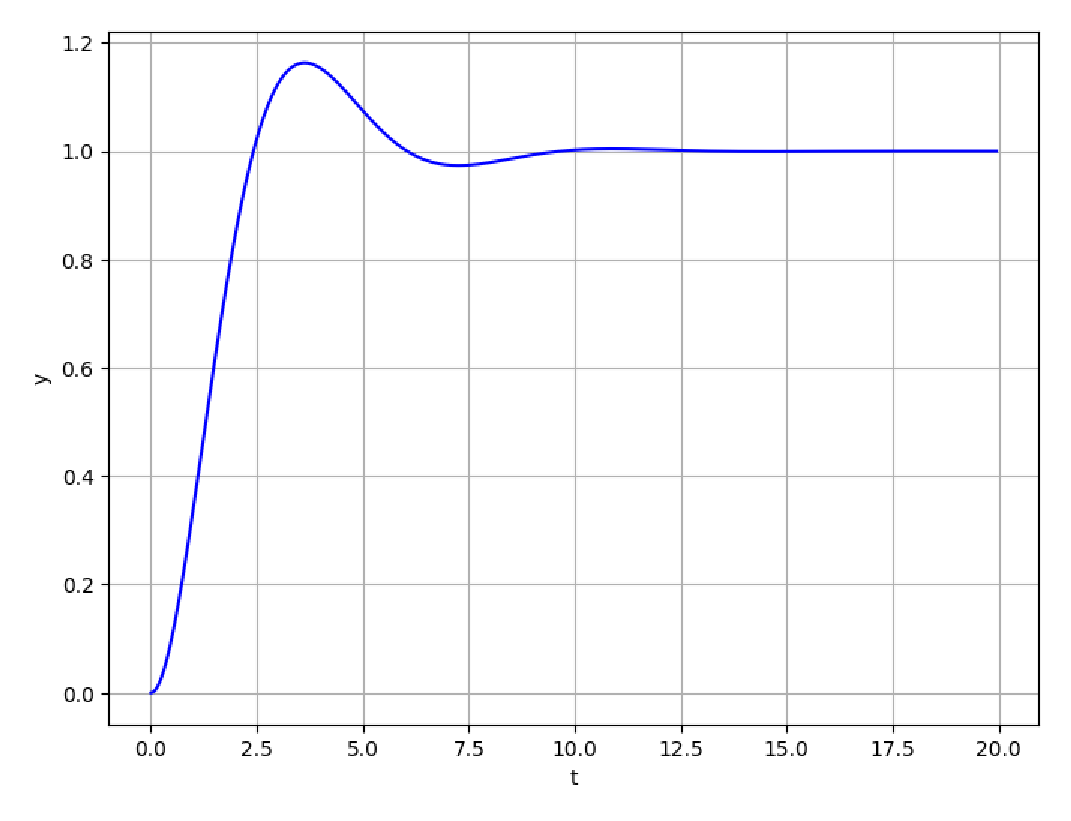
\includegraphics{figure2.eps}
  \vspace{10pt}\caption{ラダー回路の等価回路}
  \label{radder2}
\end{figure}\\
ここで、電圧源を電流源を用いて表せば図\ref{radder3}のようにできる。
\clearpage
\begin{figure}[h]
  \centering
  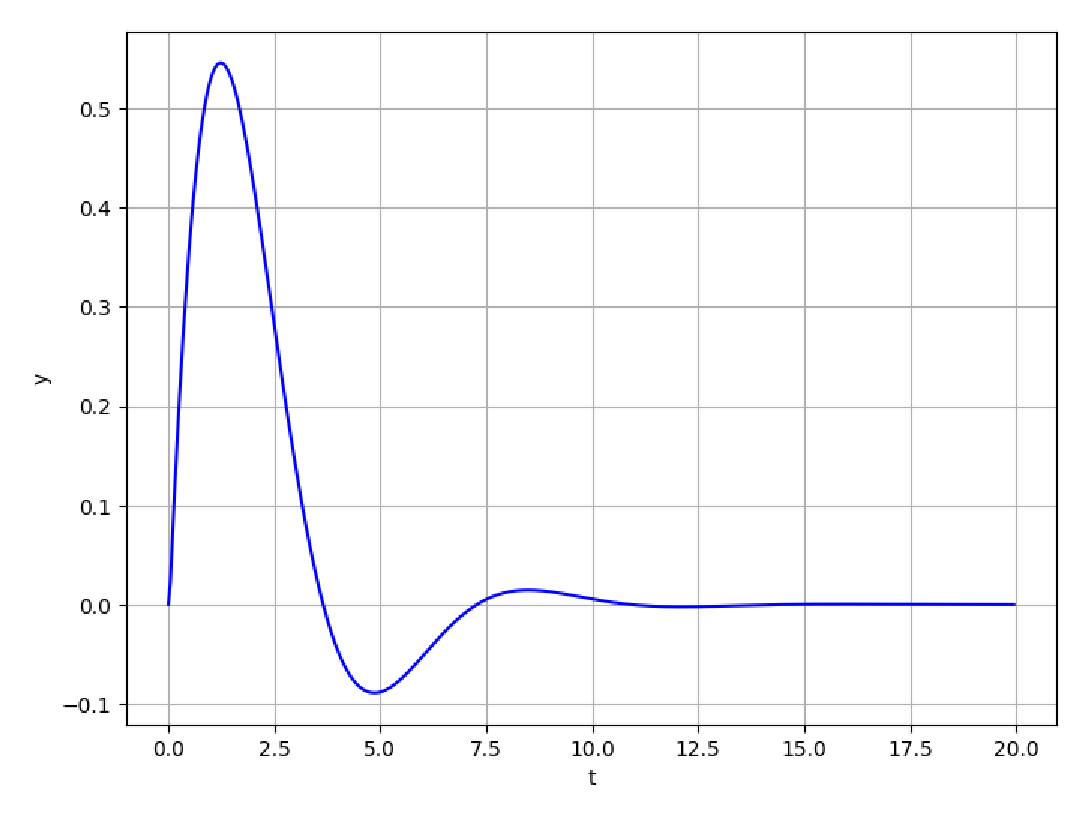
\includegraphics{figure3.eps}
  \vspace{-40pt}\caption{ラダー回路の等価回路}
  \label{radder3}
\end{figure}
先ほどの操作の逆を行うことによって図\ref{radder4}のようにできる。
\begin{figure}[h]
  \centering
  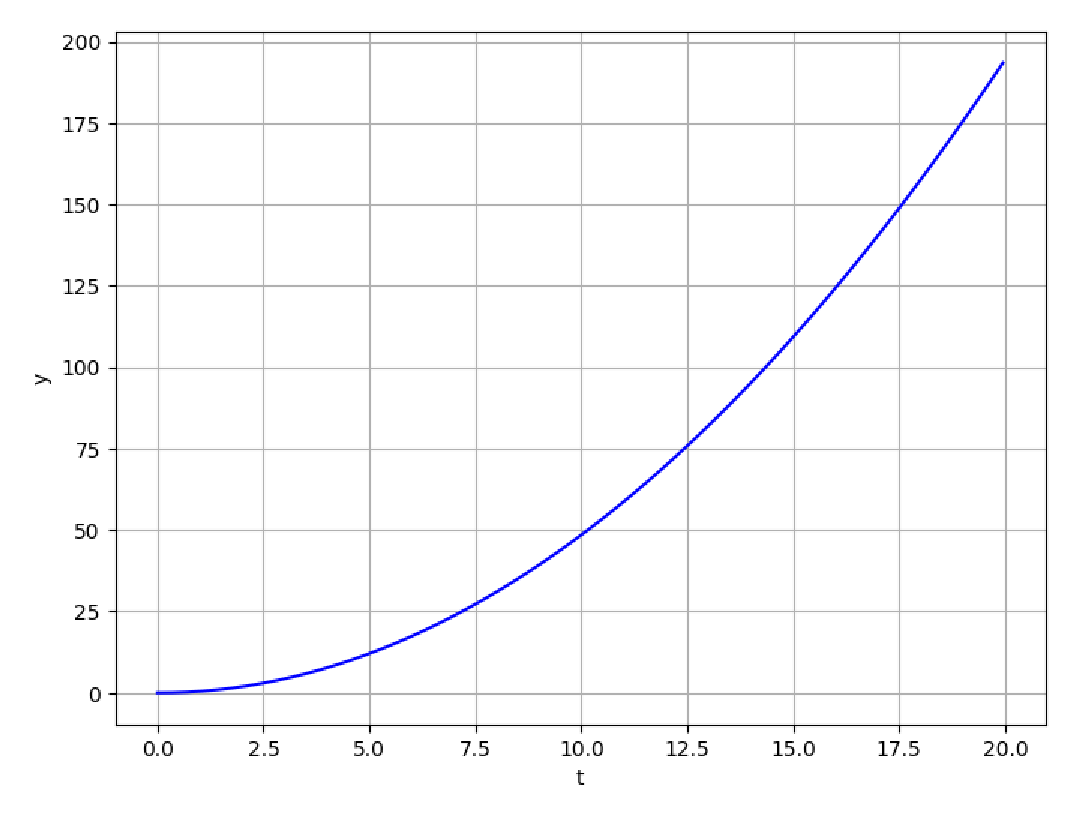
\includegraphics{figure4.eps}
  \vspace{-40pt}\caption{ラダー回路の等価回路}
  \label{radder4}
\end{figure}\\
図\ref{radder4}は図\ref{radder2}と同じ形をしていることがわかる。よって、同様の操作を繰り返すことによって図\ref{radder5}のようになる。
\clearpage
\begin{figure}[h]
  \centering
  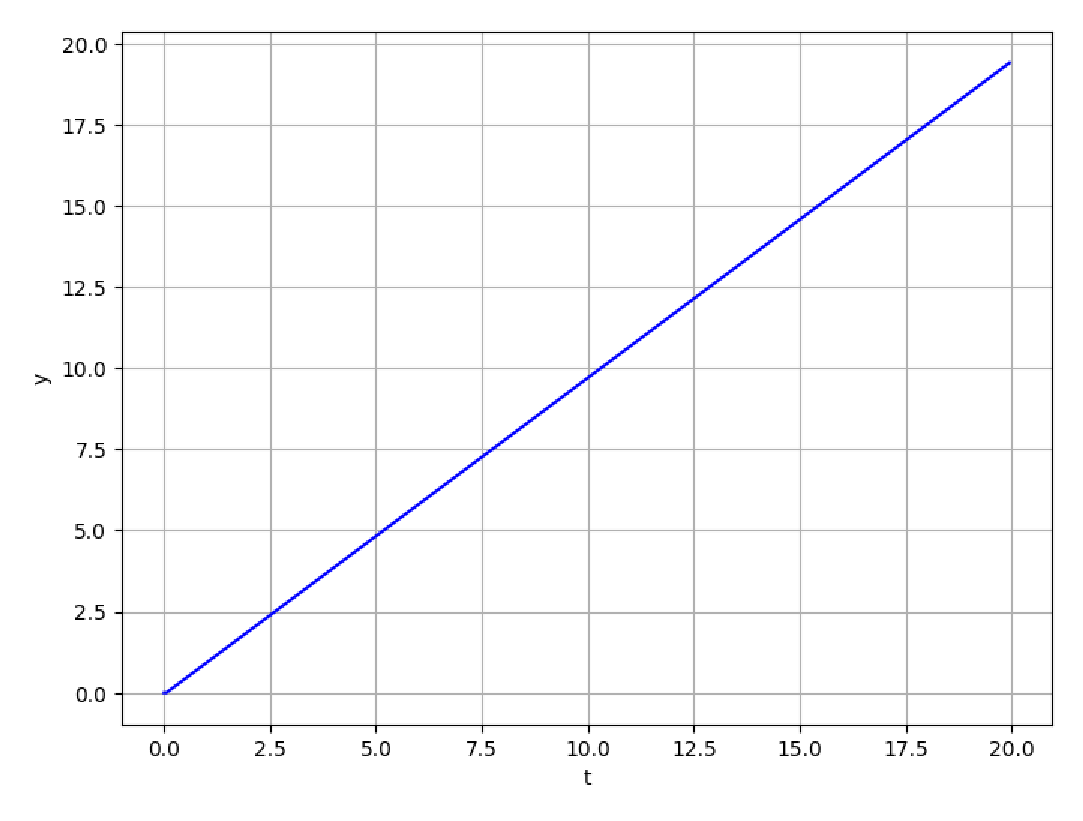
\includegraphics{figure5.eps}
  \vspace{-40pt}\caption{ラダー回路の等価回路}
  \label{radder5}
\end{figure}
図\ref{radder5}から$V^i_\mathrm{out}$を求めると
\begin{align}
  V^i_\mathrm{out}=\frac{1}{2^{n-i}}\frac{E_\mathrm{ref}}{2}
\end{align}
となる。よって、求めたい$V_\mathrm{out}$は(3)式の線形結合で表されるから、
\begin{align}
  V_\mathrm{out}=\sum^{n-1}_{i=0}2^{i-n}d_i\frac{E_\mathrm{ref}}{2}
\end{align}
となる。\\
\\
{\large \bfseries 3.2考察(f)について}\\
 マイクプリンアンプユニットとサンプルホールドユニットの間にLPFユニットを挿入する理由は、マイクから入力される信号にはノイズが多く存在するからである。普通、入力時に生じるノイズは私たちが扱いたいノイズよりも周波数がものすごく大きいことが多いためLPFユニットを用いる。また、もしLPFユニットを用いらなければノイズによって波形が大きく変化したときにサンプルホールドする場合が多くなり、サンプルホールド波形が入力波形と異なってしまう可能性が高まる。そのため、マイクプリンアンプユニットとサンプルホールドユニットの間にLPFユニットを挿入する。\\
\\
\hspace{-2pt}{\Large \bfseries 4.結論}\\
 デジタル信号の特徴を理解すると共に、アナログ信号のデジタル処理に必要なアナログ・デジタル変換の方法と性質を、実験を通じて理解することができた。\\
\\
{\Large \bfseries 参考文献}
\begin{thebibliography}{1}
\vspace{-1.5cm}
  \bibitem{text} D4実験テキスト.pdf 閲覧日:2023/12/19
  \bibitem{text1} D4実験\_補助資料2023v1.0.pdf 閲覧日:2023/12/19
  \bibitem{voice} 音の雑学大辞典,\ Pioneer\\(https:// jpn.pioneer/ja/carrozzeria/museum/oto/01\_a03.html)閲覧日:2023/12/19
\end{thebibliography}
\clearpage
$============================================================$\\
学籍番号:62115799\\
 氏  名 :平井優我\\
$============================================================$\\
■自己評価点 (100点満点): 100点 〔最低希望点: 100点〕\\
・このように評価する理由:\\自分で書いたレポートは100点じゃないとおかしい。



$------------------------------------------------------------$\\
■レポートで特に力を入れたところ:\\
全体。


$------------------------------------------------------------$\\
■レポートで難しかった・わからなかったところ:\\
なし。


$------------------------------------------------------------$\\
■レポートについて質問・確認したいこと:\\
なし。


$------------------------------------------------------------$\\
■その他の質問・意見・要望など:\\
ヘッドホンで聞いている高音質ってすごいんだなと思った。
\end{document}
